\documentclass[a4paper,11pt]{article}
\usepackage[T1]{fontenc}
\usepackage[polish]{babel}
\usepackage{lmodern,graphicx}
\usepackage[margin=2.5cm]{geometry}
\title{Wahadło: wektor i raster w publikacji}
\author{Przykład dydaktyczny}
\date{}
\begin{document}
\maketitle
\noindent Dane w \texttt{dane.csv} są syntetyczne. Punkty opisują przykładowe
okresy wahadła, a linia model $T=2\pi\sqrt{L/g}$ dla
$g=9{,}81\,\mathrm{m/s^2}$. Obie osie podają nazwę wielkości i jednostkę.
\begin{figure}[ht]
\centering
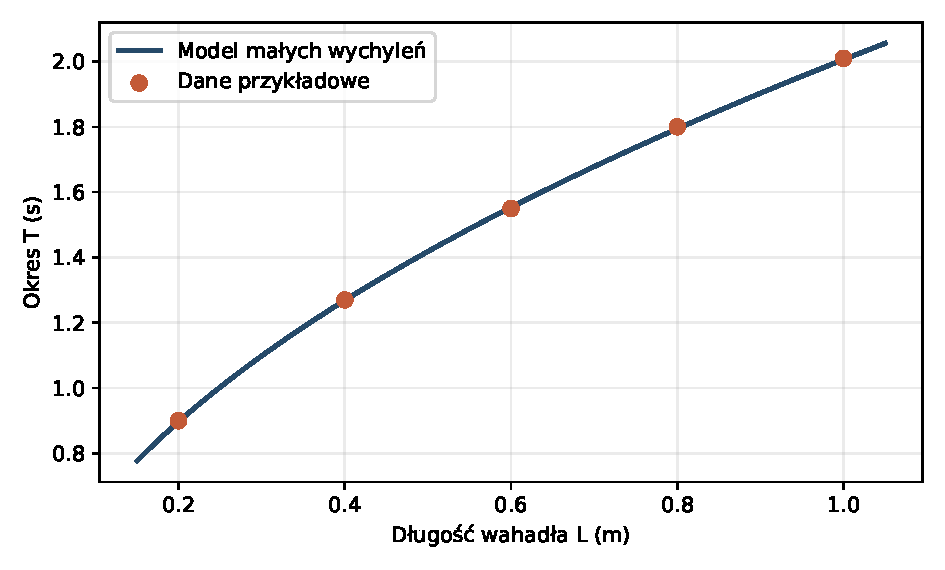
\includegraphics[width=0.92\linewidth]{wykres.pdf}
\caption{Przykładowe okresy i model małych wychyleń. Wstawiono wersję PDF.}
\end{figure}
\noindent Plik \texttt{wykres.png} ma stałą siatkę pikseli. Przy bardzo dużym
powiększeniu krawędzie tekstu i linii stają się schodkowe. W pliku
\texttt{wykres.pdf} elementy wykresu pozostają wektorowe i zachowują
ostrość przy powiększaniu; wygląd może zależeć od renderera i fontów.
PDF jest właściwym eksportem do składu LaTeX, a PNG pomaga szybko
obejrzeć rysunek w przeglądarce.
\end{document}
